\chapter{Track Finder Theory and Multivariate Classification}

Before explaining the implemented changes to the track finder for the Belle II experiment in more detail, the principles of the Belle II software framework are explained briefly. More information can be found elsewere \todo{quote}. Afterwards common figures of merit for all track finders are explained and discussed and the working principles of the already implemented track finders are illustrated. 

\section{The Belle II Analysis Framework (\texttt{basf2})}

For simulation, data acquisition, data processing and analysis of the Belle II experiment the Belle Analysis Software Framework 2 (\texttt{basf2}) is used. Although - guided by its name - it seems to be build on top of the old software framework used for the Belle experiment it is a complete rewrite of the software using modern programming principles in the coding languages C++ \cite{cpp} and Python 2.7 \cite{python}. Together with external programming libraries like ROOT \cite{root} or EvtGen \cite{evtgen} that are already on the market this framework builds the base for every software written for the experiment.

The software is divided into several packages - each serving a single purpose or summarizing code for a single detector. Examples for the packages are CDC, SVD or the tracking packaged which is described in more detail in later chapters.

Each usage of the Belle Analysis Software Framework - if it is either a simulation, a reconstruction or an analysis does not matter - consists of processing one or more so called \emph{paths} build with \emph{modules}. These modules perform a dedicated small task like simulating the hard scattering event (the so called \texttt{EvtGen} module), writing out data to a root file (the module is called \texttt{RootOutput}) or performing a track reconstruction (for example with the module \texttt{TrackFinderCDCAutomaton}). The presence, the order and the parameters of the modules are determined in \emph{steering} files written with python. The modules itself can be written in C++ or python. 

In these steering files a path is created, filled and passed to the framework which handles loading the corresponding C++ libraries and calling the modules for every event that should be processed. An example of a small steering file for track finding can be found in listing \ref{lis-steering-file}. \todo{listing} Caused by this extremely modular structure not only parallel processing but also debugging of intermediate steps can be performed much easier.

Because many modules need the data produces by other modules before there is a need for intermodular communication. This communication is performed within the framework with the help of the data store. This class as a wrapper around a collection of named \texttt{TClonesArrays} from the ROOT library \cite{tclonesarray} which can store lists of instances of nearly arbitrary C++ classes. It is used widely in the framework to store all sorts of things like the hit information produced by the particles in the simulation or the found tracks after the track finding modules. The modules have read and write access to every so called store array in the data store. A visualization of the data flow between the modules created with the steering file in \ref{lis-steering-file} can be found in figure \ref{fig-viz-datastore}. The data store can be written to or read from disk using ROOTs own serialization mechanism together with data member dictionaries for the C++ classes created by the C++ interpreter of ROOT called CINT.

\section{Working Principle of the implemented CDC Track Finder in \texttt{basf2}}

One part of this work was the improvement and further development of the track finder modules for the CDC tracking detector. Therefore the working principles of the two track finder for this detector are described here briefly. For more information on the first track finder - the legendre track finder - see \cite{kronenbitter}. More information on the second described track finder - the automaton track finder - can be found in \cite{oliver}.

The general purpose of a track finder algorithm is to partition all measured wire hits into exclusive sets of hits that may come from the same charged particle passing through the detector. It does so by using several assumptions on the charged particle producing the wire hits like the form of their trajectory and therefore the possible patterns of the hits. After fitting a mathematical model of a trajectory to these hits one can gain information on the momentum or the vertex position of this particle. There are several different approaches to find the correct sets of hits which are in the following called tracks.

The reason to have two track finders for the CDC is their different ansatz. The legendre track finder is a so called global track finder whereas the automaton track finder is a local one. A global algorithm uses the information of all wire hits simultaneously. The legendre track finder does this by applying a mathematical projection to the wire positions which should in principle project all hits belonging to the same track onto the same coordinates. A local algorithm however tries to use neighboring wire hits to construct clusters of hits. These clusters are then enlarged by using neighborhood relations until a full track can be found. In the following these two principles are described in more detail.

\subsection{The Legendre Track Finder}
The principle of using the legendre transformation for tracking algorithms in high energy particle experiments was first described by Alexopoulos \cite{legendre}. It uses an extended version of the hough transformation introduced by Paul V.V. Hough in 1962. The algorithm uses the fact that each trajectory in the $r$-$\phi$-plane of the detector can be described by a circle - assuming no energy loss - because of the applied magnetic field. In a first approximation one can also assume that each particles comes from the interaction point which is valid for the bigger part of the decay products. Therefore the trajectory in the $r$-$\phi$ direction can be described by two parameters: the radius $R$ of the circle and the angle $\phi$ between an arbitrary but fixed axis and the tangent to the circle at the interaction point.

The idea is now to transform the $x$ and $y$ coordinate pair of every axial wire hit together with the drift length $R$ with the function
\begin{align*} x' = \frac{2x}{x^2 + y^2 - R^2} \qquad y' = \frac{2y}{x^2 + y^2 - R^2}  \qquad R' = \frac{2R}{x^2 + y^2 - R^2} \end{align*}
$$r = x' \cos(\theta) + y' \sin(\theta) \pm R'$$
into the legendre space as it can be seen in figure \ref{fig-legendre-explained}. In the first step, the wire hits are transformed to the inverted plane. With this transformation each circular trajectory through the interaction point is mapped onto a line going through the origin. After that each drift circle is transformed into a pair of sinusoidal functions. This function is constructed in that way to use the fact that each trajectory of a charged particle responsible for a wire hit must touch the drift circle tangentially. Each point on the constructed sinusoidal functions correspond to one possible trajectory of a particle which could have created such a hit. The coordinates in the legendre space are the two parameters describing the trajectory as mentioned before. There are two sinusoidal functions because the osculation point can be on the far or the near side of the drift circle - the trajectory circle can contain the drift circle or not.

With using the information of a single hit one ends up with an infinite number of trajectory hypothesis. But as a charged particle passed many drift cells until it leaves the CDC detector - in some cases up to 100 hits - several wire hits are created with the same trajectory parameters. As these same parameters correspond to the same point in the legendre space, the sinusoidal functions of the wire hits intersect in this point as it can be seen in figure \ref{fig-legendre-many}. The task of the legendre algorithm is now to do the transformation of the hit coordinates and find those intersections.

Imperfections due to energy loss and material effects make the sinusoidal function not interact in one single point but rather in smeared area. To copy with this problem but still find the intersections with a good performance a peak search in the legendre space is applied. The legendre space is divided into small bins. For each bin the number of sinusoidal functions passing this area is counted. The bin with the highest weight is assumed to be the bin with the highest number of sinusoidal intersections. From the wire hits contributing to this bin a new track is created and the search is repeated until a threshold in the bin entry is undercut. As the legendre space is mostly empty this procedure can be further improved in performance by refining the bin devision from very coarse bin sizes to finer ones only for those bins which have a certain amount of sinusoidal functions in them. Because these bins are divided into 4 subbins the concept is also called a quad tree search. The whole search is depicted in figure \ref{fig-quad-tree-seach}.

\subsubsection{Stereo Hit Finding}


\subsection{The Automaton Track Finder}
Clusterizer, Automaton-Principle


\section{The used Figures Of Merit}

For testing and developing and also for later usage in the experiment setup we need to compile numbers from the implemented track finder algorithms to show how well they work. There are three different classes of figures of merit to describe a track finder. All three classes listed here are described in more detail below. The three classes are:
\begin{itemize}
  \item the efficiency (like the hit efficiency or the finding efficiency, also split up for different particle types, momentum regions or areas in the detector)
  \item the error rate (like the clone or fake rate)
  \item the computational performance (like timing and memory consumption)
\end{itemize}

The last class should be quite clear and is measured by the basf2-own measuring algorithms. As the tracking is part of the online reconstruction and may be once adopted for the high level trigger, the timing performance is very important. 

The other two classes can best be described with the algorithm how they get computed. It starts with a full Monte Carlo simulation of generic BB events with the full detector simulation afterwards. The created hits can then be parted into distinct sets - each describing a simulated tracks, called MCTrackCand (they are called track candidates to fit the naming convention of the track finder). Only those tracks are kept as a MCTrackCand, that have at least 3 hits in the CDC - otherwise they can not be fitted and even if there were a chance to find them via track finding, they could not be used for physics. After that, the simulated hits with the stripped MC information are used for track finding with the method to be evaluated. This can be done easily as the simulated hits are transformed in a format that is similar to the format that will be used later for the data coming from the experiment. After the track finder has produced a list of track candidates also, we can use the saved MC information to match tracks from the track finder to tracks from the mc algorithm (also called MC track finder) by counting the number of hits they share. The different cases are depicted and described in table \ref{tab-mc-track-finder}.

\begin{table}
  \begin{tabular}{m{0.4\linewidth}m{0.55\linewidth}} \toprule
    \centering 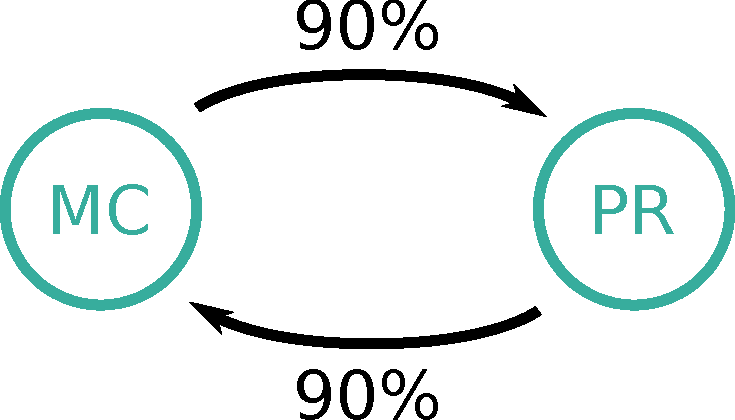
\includegraphics[width=0.8\linewidth]{figures/theory/fom_found.pdf} & There is a one to one connection between a MCTrackCand and a track from the track finder. The MCTrackCand is labeled found and the other track is labeled matched. \\ \midrule
    \centering 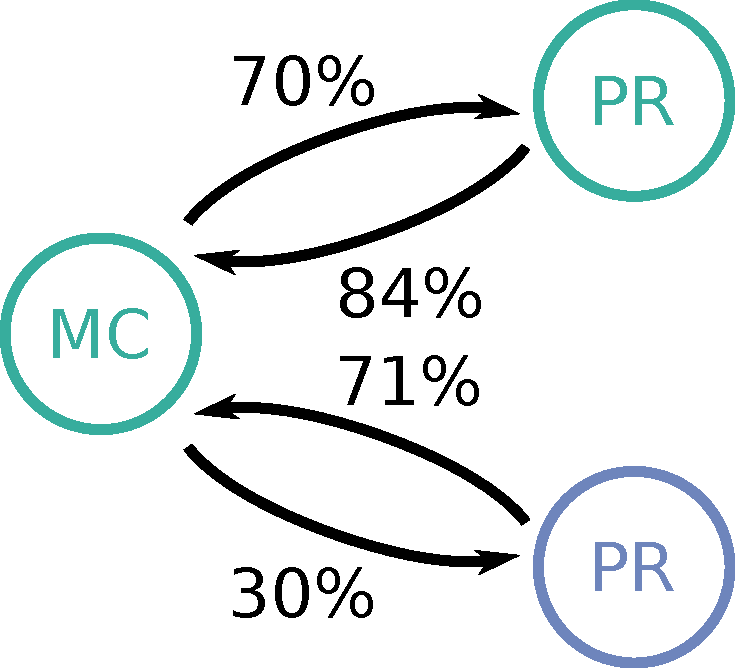
\includegraphics[width=0.8\linewidth]{figures/theory/fom_clone.pdf} & The MCTrackCand is found twice. The track from the track finder with the higher percentage (the green one in this example) is labeled matched, the other one cloned. The MCTrackCand is nevertheless labeled found. \\  \midrule
    \centering 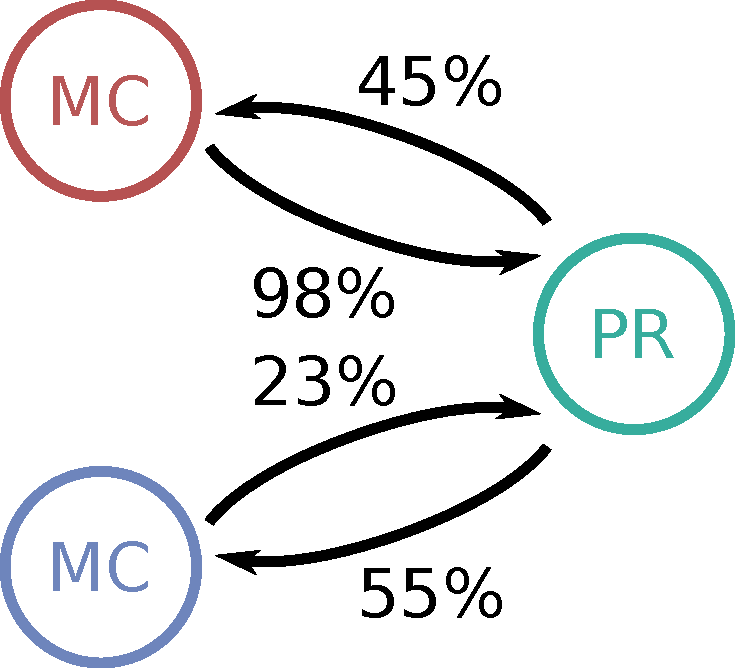
\includegraphics[width=0.8\linewidth]{figures/theory/fom_fake.pdf} & The track from the track finder is created with hits from many different MCTrackCands. As none of the corresponding hit ratios exceeds 66 \%, the track is called fake. There is no precise reason why the number 66\% was chosen. The hit ratios of the MCTrackCands itself do not play any role here. TODO: Is found for MC possible? \\  \midrule
    \centering 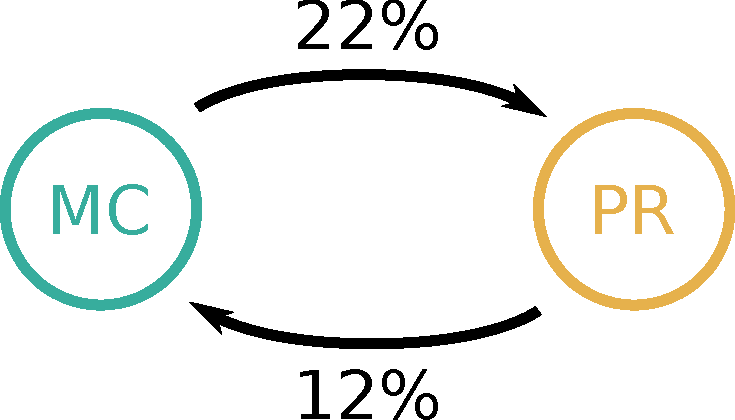
\includegraphics[width=0.8\linewidth]{figures/theory/fom_background.pdf} & The found track does not describe any of the MCTrackCands well (or well enough) - but is made out of background hits. This track is also called a fake. \\ \bottomrule
  \end{tabular}
  \caption[Matching routine for compiling the FOM.]{This tabular shows the four different cases for the matching between tracks found by the track finder (on the left side of the pictures) and MCTrackCands (shown on the right side). The different colors differentiate between different tracks. The connection between tracks shows that these two tracks share hits. The two percentages on the arrows are the percentages of hits they share in respect to the total number of hits in the MCTrackCand/track candidate from the track finder.}
  \label{tab-mc-track-finder}
\end{table}

The finding efficiency now describes the rate of MCTrackCands which are labeled matched by their total amount. Building this ratio can also be done for bins in various variables, like perpendicular momentum ($p_T$), angle in the curling plane ($phi$), number of tracks per event (multiplicity) and many more. A perfect track finder would have a finding efficiency of 100 \%. In most of the cases, the finding efficiency drops for tracks in a certain region of these variables - like for low momentum tracks.
The hit efficiency is the mean of the ratios between the number of hits in the MCTrackCands matched to a non-fake track candidate to the number of hits in total to this track. Here also a perfect track finder would have a hit efficiency of 100 \%. As in most of the cases the track finder looses some outlaying hits the hit efficiency drops.
The fake and clone rates are just the number of track candidates labeled as fake or clone by the matching algorithm divided by the number of found tracks in total. A perfect track finder would have both number set to 0 \%. A high fake rate is caused by a track finder with too loose cuts when putting together single pieces of tracks to a big track or by one which picks up background hits often. A track finder with a high clone rate on the other hand has to harsh cuts and splits up tracks into more than one piece.


\section{Multivariate Classification}
Classification, BDTs